\documentclass[11pt]{article}

\usepackage[margin=1in]{geometry}
\usepackage[T1]{fontenc}
\usepackage[utf8]{inputenc}
\usepackage{array}
\usepackage{booktabs}
\usepackage{graphicx}
\usepackage{xcolor}
\usepackage{tikz}
\usepackage[hidelinks]{hyperref}

\newcolumntype{L}[1]{>{\raggedright\arraybackslash}p{#1}}
\setlength{\floatsep}{8pt plus 2pt minus 2pt}
\setlength{\textfloatsep}{10pt plus 2pt minus 2pt}
\setlength{\intextsep}{8pt plus 2pt minus 2pt}
\setlength{\abovecaptionskip}{4pt}
\setlength{\belowcaptionskip}{2pt}
\renewcommand{\topfraction}{0.92}
\renewcommand{\bottomfraction}{0.85}
\renewcommand{\textfraction}{0.07}
\renewcommand{\floatpagefraction}{0.78}
\setcounter{topnumber}{4}
\setcounter{bottomnumber}{3}
\setcounter{totalnumber}{5}
\providecommand{\GeneratedDir}{generated}
% Generated by paper/scripts/generate_tables.py; do not edit by hand.
\newcommand{\LegislativeRowCount}{1,702}
\newcommand{\ReviewRowCount}{540}
\newcommand{\AntiCaptureRowCount}{35}
\newcommand{\SourcePaperCrosswalkCount}{4}
\newcommand{\ReviewSharedConfiguredMetricCount}{10}
\newcommand{\ReviewImportedOnlyConfiguredMetricCount}{6}
\newcommand{\ReviewCompanionOnlyConfiguredMetricCount}{2}
\newcommand{\ReviewAdaptiveCandidateCount}{16}
\newcommand{\ReviewHarmonizedMetricCount}{10}
\newcommand{\DualReviewCompanionPortfolioCount}{33,810}
\newcommand{\DualReviewTopTwentyFiveOverlap}{2}
\newcommand{\DualReviewPrimaryWinnerRankInCompanion}{not comparable}
\newcommand{\HarmonizedReviewPortfolioCount}{77,280}
\newcommand{\HarmonizedReviewTopTwentyFiveOverlap}{2}
\newcommand{\HarmonizedReviewPrimaryWinnerRank}{253}
\newcommand{\HarmonizedReviewWinnerName}{Expanded portfolio hybrid legislature + Constitutional Review Simulator: Mandatory legislative response cycles + Full anti-capture bundle}
\newcommand{\ReviewVariantRankShiftRowCount}{54}
\newcommand{\CurrentHarmonizedTopHundredOverlap}{6}
\newcommand{\PortfolioCount}{43,470}
\newcommand{\ParetoPortfolioCount}{2,730}
\newcommand{\EpsilonParetoPortfolioCount}{237}
\newcommand{\UncertaintyParetoPortfolioCount}{17,494}
\newcommand{\ScoringProfileCount}{6}
\newcommand{\BridgePeriodCount}{24}
\newcommand{\BridgeCaseCount}{7}
\newcommand{\BridgeUnmodeledPortfolioCount}{43,463}
\newcommand{\StressProfileCount}{8}
\newcommand{\AdaptiveBridgePeriodCount}{36}
\newcommand{\AdaptiveBridgePortfolioCount}{43,470}
\newcommand{\AdaptiveBridgeRunCount}{347,760}
\newcommand{\AdaptiveProvisionalShortlistCount}{0}
\newcommand{\AdaptiveCalibrationGrayZoneCount}{5,710}
\newcommand{\AdaptiveReviewPriorityCount}{0}
\newcommand{\AdaptiveDoNotRecommendCount}{37,760}
\newcommand{\AdaptiveLeaderName}{Unicameral majority + pairwise alternatives + No emergency relief without merits review + Full anti-capture bundle}
\newcommand{\AdaptiveLeaderScore}{0.709}
\newcommand{\AdaptiveLeaderWorstStressRank}{25}
\newcommand{\AdaptiveLeaderMaxStressRegret}{0.017}
\newcommand{\AdaptiveLeaderGate}{calibration gray zone, not recommendation}
\newcommand{\BalancedAdaptiveRank}{3,663}
\newcommand{\BalancedAdaptiveScore}{0.651}
\newcommand{\BalancedAdaptiveWorstStressRank}{19,816}
\newcommand{\BalancedAdaptiveMaxStressRegret}{0.168}
\newcommand{\BalancedAdaptiveGate}{do not recommend yet}
\newcommand{\RobustAdaptiveRank}{6}
\newcommand{\RobustAdaptiveScore}{0.705}
\newcommand{\RobustAdaptiveWorstStressRank}{82}
\newcommand{\RobustAdaptiveGate}{calibration gray zone, not recommendation}
\newcommand{\BalancedWinnerName}{Expanded portfolio hybrid legislature + No emergency relief without merits review + Full anti-capture bundle}
\newcommand{\BalancedWinnerScore}{0.661}
\newcommand{\BalancedWinnerUncertaintyLow}{0.569}
\newcommand{\BalancedWinnerUncertaintyHigh}{0.753}
\newcommand{\BalancedWinnerUncertaintyBand}{0.092}
\newcommand{\BalancedWinnerMinimaxRegretRank}{7,041}
\newcommand{\BalancedWinnerMaxProfileRegret}{0.107}
\newcommand{\BalancedUncertaintyOverlapCount}{43,469}
\newcommand{\BalancedUncertaintyBelowCount}{1}
\newcommand{\BalancedUncertaintyAboveCount}{0}
\newcommand{\BalancedUncertaintyLowerBoundRank}{1}
\newcommand{\UncertaintyLowerBoundWinnerName}{Expanded portfolio hybrid legislature + No emergency relief without merits review + Full anti-capture bundle}
\newcommand{\UncertaintyLowerBoundWinnerBalancedRank}{1}
\newcommand{\BalancedWinnerDelivery}{0.756}
\newcommand{\BalancedWinnerPublicAlignment}{0.537}
\newcommand{\BalancedWinnerRightsSafeguard}{0.723}
\newcommand{\BalancedWinnerCaptureResistance}{0.657}
\newcommand{\BalancedWinnerLegitimacy}{0.617}
\newcommand{\BalancedWinnerComplexity}{0.551}
\newcommand{\RobustWinnerName}{Portfolio hybrid legislature + No emergency relief without merits review + Full anti-capture bundle}
\newcommand{\RobustWinnerScore}{0.771}
\newcommand{\RobustWinnerBalancedRank}{256}
\newcommand{\RobustWinnerAverageProfileRank}{1563.333}
\newcommand{\RobustWinnerWorstProfileRank}{4,910}
\newcommand{\RobustWinnerTopTwentyFiveCount}{3}
\newcommand{\MinimaxWinnerName}{Default pass + multi-round mediation + challenge + No emergency relief without merits review + Full anti-capture bundle}
\newcommand{\MinimaxWinnerBalancedRank}{339}
\newcommand{\MinimaxWinnerMaxProfileRegret}{0.050}
\newcommand{\FragileWatchlistCount}{29}
\newcommand{\BaselineBridgeWinnerName}{Balanced winner}
\newcommand{\BaselineBridgeWinnerPortfolio}{Expanded portfolio hybrid legislature + No emergency relief without merits review + Full anti-capture bundle}
\newcommand{\BaselineBridgeWinnerScore}{0.727}
\newcommand{\BalancedBridgeScore}{0.727}
\newcommand{\BalancedBridgeAverageDelivery}{0.612}
\newcommand{\BalancedBridgeFinalPolicyQuality}{0.359}
\newcommand{\EfficiencyCautionAverageDelivery}{0.634}
\newcommand{\EfficiencyCautionFinalPolicyQuality}{0.352}
\newcommand{\EfficiencyCautionFinalPublicAlignment}{0.494}
\newcommand{\CurrentBaselineAverageDelivery}{0.288}
\newcommand{\CurrentBaselineFinalPolicyQuality}{0.000}
\newcommand{\BalancedStressWins}{5}
\newcommand{\BalancedStressTopTwo}{5}
\newcommand{\BalancedAverageStressRank}{2.250}
\newcommand{\BalancedWinTopTwoStabilityRank}{1}
\newcommand{\BalancedAverageRankStabilityRank}{1}
\newcommand{\BalancedAverageScoreStabilityRank}{4}
\newcommand{\BalancedMinimaxStressRegretRank}{4}
\newcommand{\WinTopTwoStressWinnerName}{Balanced winner}
\newcommand{\AverageRankStressWinnerName}{Balanced winner}
\newcommand{\AverageScoreStressWinnerName}{Robustness winner}
\newcommand{\MinimaxStressRegretWinnerName}{Robustness winner}
\newcommand{\ScoreSpreadStressWinnerName}{Robustness winner}
\newcommand{\HighCaptureWinnerName}{Robustness winner}
\newcommand{\HighCaptureWinnerPortfolio}{Portfolio hybrid legislature + No emergency relief without merits review + Full anti-capture bundle}
\newcommand{\BalancedHighCaptureRank}{5}
\newcommand{\BalancedEmergencyAbuseRank}{4}
\newcommand{\EmergencyAbuseWinnerName}{Robustness winner}
\newcommand{\BalancedFederalismCapacityRank}{1}
\newcommand{\LegitimacyAverageStressRank}{3.750}
\newcommand{\LegitimacyStressWins}{0}
\newcommand{\LegitimacyStressTopTwo}{1}
\newcommand{\EfficiencyCautionStressWins}{0}
\newcommand{\EfficiencyCautionAverageStressRank}{4.625}


\title{Institutional Portfolios for Efficient Democratic Government}
\author{}
\date{\today}

\begin{document}
\maketitle

\begin{abstract}
This working paper asks what can be learned by combining the legislative, constitutional-review, and lobbying/capture simulator projects into one portfolio screen. The current revision rechecks \SourcePaperCrosswalkCount{} updated sibling papers and report artifacts, then imports \LegislativeRowCount{} legislative campaign rows, \ReviewRowCount{} constitutional-review rows, and \AntiCaptureRowCount{} lobbying/capture rows, producing \PortfolioCount{} primary institutional portfolios. It does not treat every updated review artifact as interchangeable. Instead, it builds a review harmonization manifest, a companion review-source swap, and a conservative harmonized review source with \ReviewHarmonizedMetricCount{} shared static metrics. The harness then runs a focused \BridgePeriodCount-period interbranch bridge model over \BridgeCaseCount{} selected cases and a synthetic \AdaptiveBridgePeriodCount-period adaptive bridge over all \AdaptiveBridgePortfolioCount{} primary portfolios. The result is not a settled recommendation. Several candidate portfolios beat the stylized current-system baseline in the current synthetic screens, but no portfolio yet passes the adaptive recommendation gate. The balanced winner remains the leading static point-estimate and lower-bound candidate, while Adaptive Bridge v1 marks it \BalancedAdaptiveGate. The best use of the paper is therefore screening: narrow the design space, expose fragile winners, and specify the validation work needed before institutional recommendations are made.
\end{abstract}

\section{Research Question}

The question is not which single institution looks strongest in isolation. The question is which combinations preserve public lawmaking capacity while preventing predictable institutional failure modes:

\begin{itemize}
  \item low-support or weak-mandate policy passage;
  \item rights-threatening laws or emergency actions;
  \item lobbying capture, dark influence, and reform evasion;
  \item constitutional instability and interbranch conflict;
  \item excessive administrative cost or procedural complexity.
\end{itemize}

The object of comparison is therefore the institutional portfolio: one legislative design, one review design, and one anti-capture design evaluated together.

The contribution is narrower than a constitutional blueprint. The paper shows how separately calibrated simulators can be combined without pretending they form one statistical model. It uses the combined screen to sort candidate families, identify fragile headline winners, and state what evidence would be required before stronger claims are justified.

\section{Argument Map}

The body keeps only claims that change how a skeptical reader should interpret the results. Other diagnostic material is moved to the appendix.

\begin{center}
\small
\begin{tabular}{@{}L{0.20\linewidth}L{0.36\linewidth}L{0.34\linewidth}@{}}
\toprule
Claim role & Evidence used in the body & Permitted conclusion \\
\midrule
Source scope & Imported rows, provenance, and sibling-paper crosswalk & The paper is a synthesis of three imported simulator families, with one updated constitutional-review companion used as a scope-control cross-check. \\
Static screen & Balanced score, uncertainty overlap, and the focused candidate comparison & Some portfolios outperform the stylized current-system baseline, but rank one is not uncertainty-resolved. \\
Feedback stress & Focused bridge v0 and stress exceptions & Candidate families must be judged by adaptation pressure, not only static efficiency. \\
Recommendation boundary & Adaptive Bridge v1 gate counts and validation agenda & Current winners are validation targets, not settled institutional recommendations. \\
\bottomrule
\end{tabular}
\end{center}

The paper separates three claim types. Empirical-source claims are limited to the imported report artifacts and their recorded provenance. Synthetic findings are claims produced by cumulative scoring, regret, Pareto, robustness, and bridge layers. Speculative design recommendations are proposals for future model extensions, calibration work, or reform sequences that are not yet tested as portfolio rows or bridge mechanisms.

\section{Evidence Base}

The cumulative project imports three existing simulator families and cross-references one updated companion review project. The Congress Institutional Simulator contributes lawmaking capacity, public alignment, welfare, gridlock, legitimacy, concentrated-harm passage, lobbying pressure, and administrative-feasibility diagnostics. The Supreme Court Simulator Design project contributes rights protection, review stability, democratic responsiveness, emergency abuse control, independence/accountability balance, legitimacy, public confidence, constitutional conflict, and cost diagnostics. The Lobby Capture Simulator contributes capture control, representation, public-interest alignment, detection, sanctioning, net transparency, hidden influence, reform decay, and administrative-cost diagnostics.

The updated Constitutional Review Simulator now contributes a stronger comparative-review check on the paper's interpretation. It is not folded into the primary ranking as if it were just more rows from the same simulator, because it overlaps the imported review family while using different case structures, denominators, and additional compliance, implementation, defiance, emergency, and public-trust fields. A naive concatenation would overstate certainty. The current build therefore separates three objects: the primary imported Supreme Court Design source, a companion Constitutional Review source swap, and a conservative harmonized review source that includes only same-name, same-direction, defensibly comparable static review fields.

% Generated by paper/scripts/generate_tables.py; do not edit by hand.
\begin{table}[!htbp]
\centering
\footnotesize
\begin{tabular}{@{}L{0.25\linewidth}r r r L{0.34\linewidth}@{}}
\toprule
Source & Rows & Scenarios & Metrics & Imported report \\
\midrule
Congress Institutional Simulator & 1,428 & 42 & 18 & \texttt{simulation-\allowbreak{}campaign-\allowbreak{}v21-\allowbreak{}paper.csv} \\
Supreme Court Simulator Design & 520 & 26 & 18 & \texttt{constitutional-\allowbreak{}review-\allowbreak{}campaign-\allowbreak{}v2.csv} \\
Lobby Capture Simulator & 31 & 31 & 21 & \texttt{lobby-\allowbreak{}capture-\allowbreak{}campaign.csv} \\
\bottomrule
\end{tabular}
\caption{Current source artifacts imported by the cumulative harness.}
\end{table}

% Generated by paper/scripts/generate_tables.py; do not edit by hand.
\begin{table}[!htbp]
\centering
\scriptsize
\setlength{\tabcolsep}{3pt}
\begin{tabular}{@{}L{0.13\linewidth}L{0.18\linewidth}L{0.16\linewidth}L{0.15\linewidth}L{0.23\linewidth}@{}}
\toprule
Project & Updated paper checked & Current report artifact & Cumulative use & Reading rule after refresh \\
\midrule
Congress Institutional Simulator & Searching Legislative Design Space for Compromise and Productivity; \texttt{main.tex}; hash \texttt{2791c54c98b5} & \texttt{simulation-\allowbreak{}campaign-\allowbreak{}v21-\allowbreak{}paper.csv}; 1,428 rows; hash \texttt{1e36005c54d3} & Imported legislative source. & Treat the updated portfolio-hybrid legislature as a synthesized candidate; pairwise alternatives remain the cleaner non-default productivity and compromise comparator. \\
Supreme Court Simulator Design & Designing Constitutional Review Institutions by Simulation; \texttt{main.tex}; hash \texttt{eef2eeba51e1} & \texttt{constitutional-\allowbreak{}review-\allowbreak{}campaign-\allowbreak{}v2.csv}; 520 rows; hash \texttt{2278a169405c} & Imported constitutional-review source. & Keep review metrics pathway-specific and proxy-aware; the updated denominator audit does not permit pooled validation claims. \\
Constitutional Review Simulator & When Constitutional Review Improves Democratic Constitutionalism: A Comparative Simulation Framework; \texttt{main.tex}; hash \texttt{dc9291f0876e} & \texttt{constitutional-\allowbreak{}review-\allowbreak{}sensitivity-\allowbreak{}v1.csv}; 231 rows; hash \texttt{dc638127a5c1} & Referenced review cross-check; not imported into rankings yet. & Use the richer compliance, defiance, implementation, emergency, and public-trust fields to guide schema reconciliation before any row merge. \\
Lobby Capture Simulator & Strategic Channel Substitution and Regulatory Capture: A Simulation Model of Lobbying and Anti-Capture Reform; \texttt{main.tex}; hash \texttt{72e62312fe3c} & \texttt{lobby-\allowbreak{}capture-\allowbreak{}campaign.csv}; 31 rows; hash \texttt{8e1e313e166c} & Imported anti-capture source. & Read low observed capture through total distortion, hidden influence, venue-shifting, and validation partial/miss diagnostics. \\
\bottomrule
\end{tabular}
\caption{Crosswalk from updated sibling simulator papers and reports to the cumulative synthesis. The Constitutional Review Simulator is deliberately treated as a review cross-check until its richer schema is reconciled with the imported Supreme Court Simulator Design campaign.}
\end{table}

% Generated by paper/scripts/generate_tables.py; do not edit by hand.
\begin{table}[!htbp]
\centering
\small
\begin{tabular}{@{}L{0.54\linewidth}r@{}}
\toprule
Review reconciliation category & Count \\
\midrule
shared configured metric & 10 \\
imported-only configured metric & 6 \\
companion-only configured metric & 2 \\
missing from both review sources & 0 \\
companion adaptive candidate & 16 \\
\bottomrule
\end{tabular}
\caption{Construct-level reconciliation between the imported Supreme Court Simulator Design review source and the companion Constitutional Review Simulator. Companion adaptive candidates are not added to the static ranking until denominator and construct ownership are resolved.}
\end{table}

% Generated by paper/scripts/generate_tables.py; do not edit by hand.
\begin{table}[!htbp]
\centering
\small
\begin{tabular}{@{}L{0.58\linewidth}r@{}}
\toprule
Harmonization action & Manifest rows \\
\midrule
included & 20 \\
excluded & 8 \\
not present & 8 \\
adaptive candidate & 16 \\
\bottomrule
\end{tabular}
\caption{Review harmonization manifest. Included static fields are: constitutionalConflict, democraticResponsiveness, directionalScore, independenceAccountabilityBalance, legalStability, legitimacy, partisanAlignment, reversalRate, rightsProtection, shadowDocketAbuse. Source-specific fields remain available in source-swap sensitivity screens or adaptive calibration work, but are excluded from the harmonized static source.}
\end{table}


The reconciliation report finds \ReviewSharedConfiguredMetricCount{} shared configured review metrics, \ReviewImportedOnlyConfiguredMetricCount{} imported-only configured metrics, \ReviewCompanionOnlyConfiguredMetricCount{} companion-only configured metrics, and \ReviewAdaptiveCandidateCount{} companion fields that are better treated as adaptive inputs unless their denominators are harmonized. The manifest admits \ReviewHarmonizedMetricCount{} static metrics into the harmonized source and excludes source-specific composites, public-confidence/cost fields, and compliance fields from the harmonized static score. The integration problem is therefore not just missing data. It is construct ownership. These source simulators were calibrated separately, so the cumulative score cannot be read as a single unified statistical estimate. It is a structured comparison across separately generated artifacts. The source-paper crosswalk records which updated artifacts are imported, cross-checked, and harmonized. For that reason, the paper treats scores as screening evidence and then checks whether the same candidates survive uncertainty, value-profile, bridge, stress, adaptive, and review-source filters.

\section{Cumulative Method}

The cumulative harness groups each source report by scenario, computes component scores from available columns, and builds every legislature-review-anti-capture combination. It then compares portfolios on delivery, public alignment, rights safeguard, capture resistance, legitimacy, efficiency, complexity, and resilience floor. The resilience floor is deliberately conservative: a portfolio that performs well in two subsystems but collapses in capture resistance, rights protection, or complexity should not outrank a more balanced package without an explicit normative reason.

The harness reports \ScoringProfileCount{} scoring profiles plus complementary Pareto, robustness, bridge, and bridge-sensitivity views. This matters because a single blended score can hide the strongest design lesson: different constitutional values reward different institutional packages, and some high-throughput packages look worse once rights, capture, legitimacy, and implementation constraints are treated as floors.

\section{Which Designs Beat the Current-System Baseline?}

The phrase ``beat the current system'' has a narrow meaning here. The current-system-ish row is a stylized benchmark assembled from the imported simulator families. It is not an empirical claim about the live U.S. constitutional order. A candidate beats that row only when it performs better in the current synthetic screens.

% Generated by paper/scripts/generate_tables.py; do not edit by hand.
\begin{table}[!htbp]
\centering
\scriptsize
\resizebox{\linewidth}{!}{%
\begin{tabular}{@{}L{0.18\linewidth}L{0.24\linewidth}L{0.20\linewidth}L{0.20\linewidth}L{0.28\linewidth}@{}}
\toprule
Candidate & Why it is in the paper & Static screen & Feedback/adaptive screen & Paper status \\
\midrule
Current-system-ish baseline & Stylized comparator, not an empirical claim about the live U.S. system. & rank 33,486; score 0.500; floor 0.419 & bridge 7/7 (0.474); adaptive rank 14,704 & Does not beat the leading synthetic portfolios; kept to show the comparison floor. \\
Balanced static winner & Best point-estimate and lower-bound static screen. & rank 1; score 0.656; max regret 0.107 & bridge 1/7 (0.723); adaptive rank 3,320 & Beats the stylized baseline in static and focused-bridge screens, but gate is do not recommend yet. \\
Robustness challenger & Best cross-profile robustness row and strongest stress-regret challenger. & balanced rank 267; robustness rank 1; floor 0.635 & bridge 6/7 (0.709); adaptive rank 7 & Stronger validation target than the static winner under adaptive screening; gate is calibration gray zone, not recommendation. \\
Adaptive gray-zone leader & Highest all-portfolio adaptive-survival score. & static rank 125; score 0.640; max regret 0.083 & bridge 4/7 (0.713); adaptive rank 1 & Best current validation target, not a recommendation; gate is calibration gray zone, not recommendation. \\
\bottomrule
\end{tabular}
}
\caption{Reader-facing synthesis of the stylized current-system baseline and the main challenger portfolios. ``Beats'' means stronger in the current synthetic screens, not empirically proven superior.}
\end{table}


The central result is that the stylized baseline is not competitive in the combined screen, while the leading alternatives separate into different roles. The balanced static winner is the best headline screen result. The robustness challenger is the stronger validation target once profile durability and stress regret matter. The adaptive gray-zone leader is the best all-portfolio adaptive screen result. None of those labels is a recommendation, because the adaptive gate produces \AdaptiveProvisionalShortlistCount{} provisional shortlist rows and \AdaptiveCalibrationGrayZoneCount{} calibration gray-zone rows.

\section{Static Finding}

The balanced-score winner is:

\begin{quote}
\BalancedWinnerName.
\end{quote}

% Generated by paper/scripts/generate_tables.py; do not edit by hand.
\begin{table}[!htbp]
\centering
\small
\begin{tabular}{@{}L{0.24\linewidth}L{0.66\linewidth}@{}}
\toprule
Portfolio component & Selected design \\
\midrule
Legislature & Expanded portfolio hybrid legislature \\
Review & No emergency relief without merits review \\
Anti-capture & Full anti-capture bundle \\
\bottomrule
\end{tabular}
\qquad
\begin{tabular}{@{}L{0.25\linewidth}r@{}}
\toprule
Diagnostic & Value \\
\midrule
Balanced score & 0.656 \\
Policy delivery & 0.745 \\
Public alignment & 0.534 \\
Rights safeguard & 0.724 \\
Capture resistance & 0.648 \\
Legitimacy & 0.613 \\
Complexity score & 0.554 \\
Resilience floor & 0.554 \\
\bottomrule
\end{tabular}
\caption{Balanced-score winner and diagnostics.}
\end{table}


Its balanced score is \BalancedWinnerScore. The diagnostic pattern is strong delivery (\BalancedWinnerDelivery), strong rights safeguard (\BalancedWinnerRightsSafeguard), moderate capture resistance (\BalancedWinnerCaptureResistance), moderate legitimacy (\BalancedWinnerLegitimacy), moderate complexity score (\BalancedWinnerComplexity), and lower public alignment (\BalancedWinnerPublicAlignment). It is a plausible headline candidate under the point-estimate score because it does not rely on one institutional mechanism alone. It combines a high-capacity legislative portfolio, a review rule that sharply restrains emergency relief, and a lobbying environment that allows access under stronger anti-capture controls.

The weakness is public alignment. The balanced winner should not be framed as a fully representative ideal. It is better described as a high-delivery, high-rights-screen portfolio with adequate capture control and manageable complexity. Its synthetic uncertainty interval is \BalancedWinnerUncertaintyLow--\BalancedWinnerUncertaintyHigh{} around the current score, with half-width \BalancedWinnerUncertaintyBand. Its lower-bound rank is \BalancedUncertaintyLowerBoundRank{}, but \BalancedUncertaintyOverlapCount{} portfolios overlap its interval. Its minimax-regret rank is \BalancedWinnerMinimaxRegretRank{} and its maximum profile regret is \BalancedWinnerMaxProfileRegret. Those diagnostics keep it in the lead under current scoring, but they prevent treating the rank-one row as uncertainty-resolved.

The uncertainty bands below are not empirical confidence intervals. They are conservative model-sensitivity bands. They widen when a portfolio combines separately calibrated source artifacts, shows component imbalance, has cross-profile instability, or depends on thin metric coverage.

% Generated by paper/scripts/generate_tables.py; do not edit by hand.
\begin{table}[!htbp]
\centering
\small
\begin{tabular}{@{}L{0.38\linewidth}L{0.52\linewidth}@{}}
\toprule
Uncertainty diagnostic & Value \\
\midrule
Balanced interval & 0.563--0.748 \\
Rows overlapping balanced interval & 33,852 \\
Rows entirely below balanced interval & 0 \\
Rows entirely above balanced interval & 0 \\
Balanced lower-bound rank & 1 \\
Lower-bound leader & Expanded portfolio hybrid legislature + No emergency relief without merits review + Full anti-capture bundle (balanced rank 1) \\
\bottomrule
\end{tabular}
\caption{Interval-resolution diagnostics for all 33,852 portfolios. Overlap counts show whether point-estimate ranks are separated by the synthetic uncertainty bands.}
\end{table}


The interval-resolution diagnostic is severe: \BalancedUncertaintyOverlapCount{} generated portfolios overlap the balanced winner's interval. The lower-bound ordering still places \UncertaintyLowerBoundWinnerName{} first, but the project should describe that as a robustness clue, not as statistical separation from the field.

The most robust cross-profile portfolio is:

\begin{quote}
\RobustWinnerName.
\end{quote}

It ranks only \RobustWinnerBalancedRank{} under the balanced score, but it has the best cross-profile durability: average profile rank \RobustWinnerAverageProfileRank, worst profile rank \RobustWinnerWorstProfileRank, and top-25 placement in \RobustWinnerTopTwentyFiveCount{} of the \ScoringProfileCount{} scoring profiles. Substantively, that points toward a design hypothesis: structured alternative selection may be more robust than a broad expanded hybrid when the evaluator cares about legitimacy, rights, and anti-capture goals as much as headline delivery. Adaptive Bridge v1 also ranks this robustness candidate much higher than the static balanced winner: adaptive rank \RobustAdaptiveRank{} versus \BalancedAdaptiveRank.

The balanced winner itself remains provisional because it has weak public-alignment diagnostics and falls far under at least one value profile. The efficiency and minimax-regret leaders are more fragile: they reduce regret or increase throughput, but their default-passage structure makes them vulnerable to weak-floor, rights, legitimacy, or capture concerns. These rows are useful for learning what the scoring model rewards; they are not ready as constitutional recommendations.

\section{Feedback and Stress Findings}

The bridge model moves the project beyond static combination, but only for a focused candidate set. It selects \BridgeCaseCount{} cases from \PortfolioCount{} static portfolios: balanced winner, minimax-regret winner, robustness winner, rights/capture winner, legitimacy-first winner, efficiency caution case, and current-system-ish baseline. The remaining \BridgeUnmodeledPortfolioCount{} static portfolios are not bridge-simulated in this paper workflow.

% Generated by paper/scripts/generate_tables.py; do not edit by hand.
\begin{table}[!htbp]
\centering
\small
\begin{tabular}{@{}rL{0.34\linewidth}r r r r@{}}
\toprule
Rank & Case & Score & Avg. delivery & Final quality & Final alignment \\
\midrule
1 & Balanced winner & 0.723 & 0.601 & 0.350 & 0.516 \\
2 & Efficiency caution case & 0.719 & 0.627 & 0.345 & 0.490 \\
3 & Minimax-regret winner & 0.715 & 0.595 & 0.337 & 0.505 \\
4 & Rights/capture winner & 0.713 & 0.528 & 0.305 & 0.507 \\
5 & Legitimacy-first winner & 0.713 & 0.528 & 0.305 & 0.507 \\
6 & Robustness winner & 0.709 & 0.516 & 0.298 & 0.507 \\
7 & Current-system-ish baseline & 0.474 & 0.297 & 0.000 & 0.195 \\
\bottomrule
\end{tabular}
\caption{Baseline interbranch bridge ranking.}
\end{table}

% Generated by paper/scripts/generate_tables.py; do not edit by hand.
\begin{figure}[!htbp]
\centering
\resizebox{0.92\linewidth}{!}{%
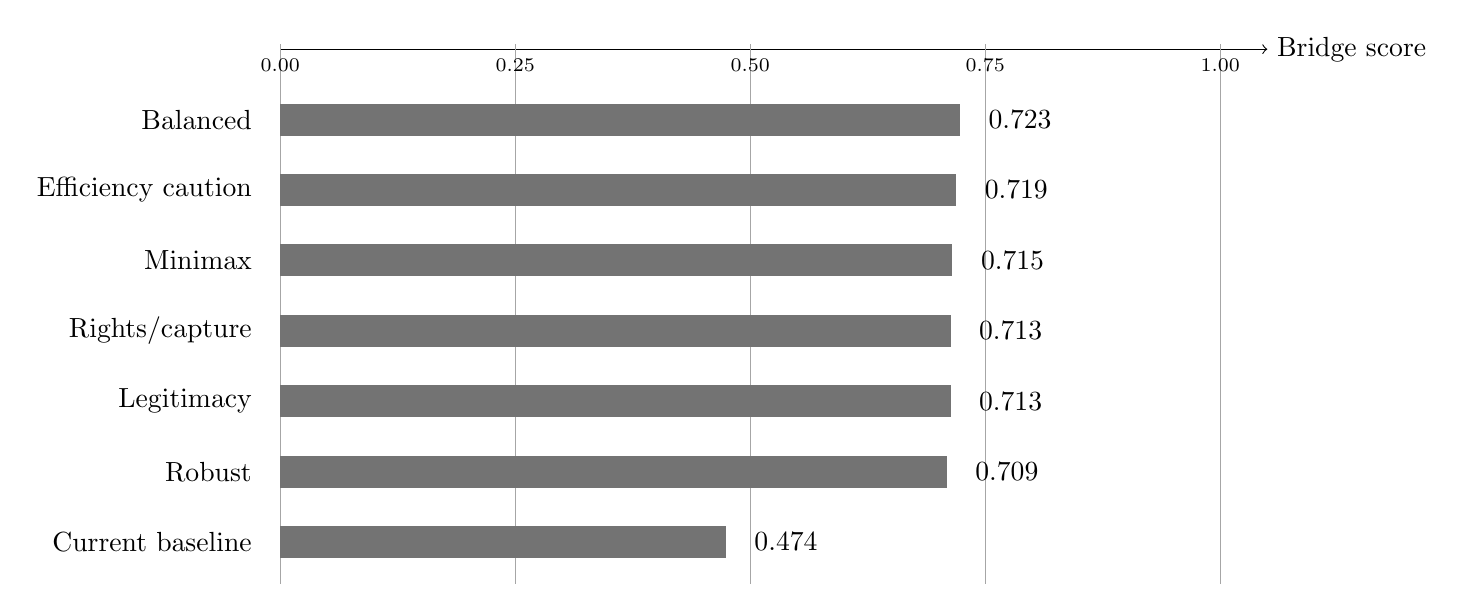
\begin{tikzpicture}[x=4.7in,y=0.80in]
\draw[->] (0,0) -- (1.05,0) node[anchor=west] {Bridge score};
\foreach \x/\lab in {0/0.00,0.25/0.25,0.50/0.50,0.75/0.75,1.00/1.00} {
  \draw[black!35] (\x,0.03) -- (\x,-3.34);
  \node[anchor=north] at (\x,0) {\scriptsize \lab};
}
\node[anchor=east] at (-0.02,-0.44) {Balanced};
\fill[black!55] (0,-0.54) rectangle (0.723,-0.34);
\node[anchor=west] at (0.743,-0.44) {0.723};
\node[anchor=east] at (-0.02,-0.88) {Efficiency caution};
\fill[black!55] (0,-0.98) rectangle (0.719,-0.78);
\node[anchor=west] at (0.739,-0.88) {0.719};
\node[anchor=east] at (-0.02,-1.32) {Minimax};
\fill[black!55] (0,-1.42) rectangle (0.715,-1.22);
\node[anchor=west] at (0.735,-1.32) {0.715};
\node[anchor=east] at (-0.02,-1.76) {Rights/capture};
\fill[black!55] (0,-1.86) rectangle (0.713,-1.66);
\node[anchor=west] at (0.733,-1.76) {0.713};
\node[anchor=east] at (-0.02,-2.20) {Legitimacy};
\fill[black!55] (0,-2.30) rectangle (0.713,-2.10);
\node[anchor=west] at (0.733,-2.20) {0.713};
\node[anchor=east] at (-0.02,-2.64) {Robust};
\fill[black!55] (0,-2.74) rectangle (0.709,-2.54);
\node[anchor=west] at (0.729,-2.64) {0.709};
\node[anchor=east] at (-0.02,-3.08) {Current baseline};
\fill[black!55] (0,-3.18) rectangle (0.474,-2.98);
\node[anchor=west] at (0.494,-3.08) {0.474};
\end{tikzpicture}
}
\caption{Baseline bridge scores for the focused portfolio cases.}
\end{figure}


Within that focused set, the baseline bridge winner is \BaselineBridgeWinnerName:

\begin{quote}
\BaselineBridgeWinnerPortfolio.
\end{quote}

This matters because the earlier robustness result could have suggested replacing the balanced winner with the pairwise-alternatives family. Focused bridge v0 does not support that as a clean replacement under baseline assumptions. Instead, it shows a tight top cluster. The balanced winner keeps more average delivery (\BalancedBridgeAverageDelivery) and the highest final policy quality in the baseline bridge run (\BalancedBridgeFinalPolicyQuality), while the minimax, legitimacy, robustness, and rights/capture cases remain close enough that the bridge should be read as a comparison-set filter rather than as a global portfolio ranking.

The current-system-ish baseline performs worst in baseline bridge v0. It has low average delivery (\CurrentBaselineAverageDelivery), final policy quality of \CurrentBaselineFinalPolicyQuality, and the report flags weak starting floor, low policy quality, public-alignment erosion, and delivery bottleneck. This result should be treated as a stylized baseline comparison, not as an empirical claim about any real constitution.

Bridge v0 reruns the same \BridgeCaseCount{} cases under \StressProfileCount{} configured stress profiles. By the configured wins/top-two rule, the balanced winner ranks first: it wins \BalancedStressWins{} of \StressProfileCount{} stress profiles, places top-two in \BalancedStressTopTwo, and has average stress rank \BalancedAverageStressRank. The stability conclusion still depends on the rule. \AverageScoreStressWinnerName{} has the best average bridge score and \MinimaxStressRegretWinnerName{} has the lowest maximum stress regret, so wins/top-two should not be described as the only defensible stability criterion.

% Generated by paper/scripts/generate_tables.py; do not edit by hand.
\begin{figure}[!htbp]
\centering
\resizebox{0.92\linewidth}{!}{%
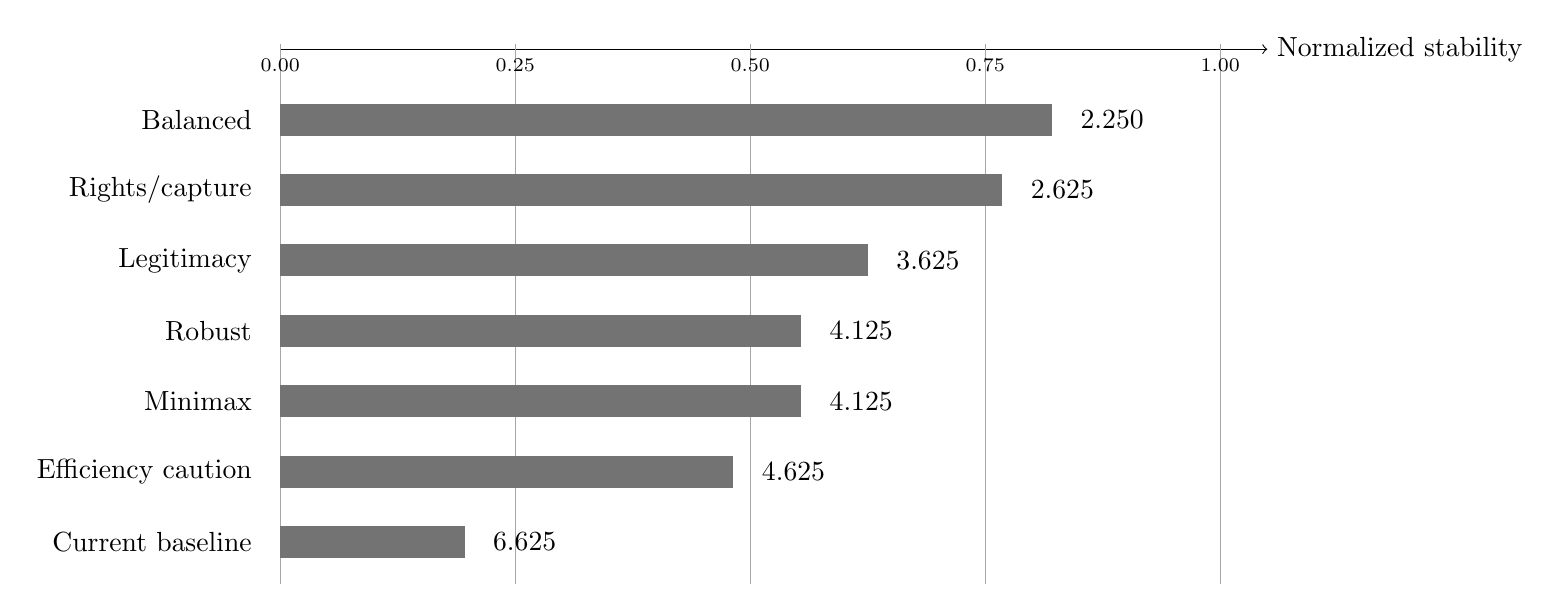
\begin{tikzpicture}[x=4.7in,y=0.80in]
\draw[->] (0,0) -- (1.05,0) node[anchor=west] {Normalized stability};
\foreach \x/\lab in {0/0.00,0.25/0.25,0.50/0.50,0.75/0.75,1.00/1.00} {
  \draw[black!35] (\x,0.03) -- (\x,-3.34);
  \node[anchor=north] at (\x,0) {\scriptsize \lab};
}
\node[anchor=east] at (-0.02,-0.44) {Balanced};
\fill[black!55] (0,-0.54) rectangle (0.821,-0.34);
\node[anchor=west] at (0.841,-0.44) {2.250};
\node[anchor=east] at (-0.02,-0.88) {Rights/capture};
\fill[black!55] (0,-0.98) rectangle (0.768,-0.78);
\node[anchor=west] at (0.788,-0.88) {2.625};
\node[anchor=east] at (-0.02,-1.32) {Legitimacy};
\fill[black!55] (0,-1.42) rectangle (0.625,-1.22);
\node[anchor=west] at (0.645,-1.32) {3.625};
\node[anchor=east] at (-0.02,-1.76) {Robust};
\fill[black!55] (0,-1.86) rectangle (0.554,-1.66);
\node[anchor=west] at (0.574,-1.76) {4.125};
\node[anchor=east] at (-0.02,-2.20) {Minimax};
\fill[black!55] (0,-2.30) rectangle (0.554,-2.10);
\node[anchor=west] at (0.574,-2.20) {4.125};
\node[anchor=east] at (-0.02,-2.64) {Efficiency caution};
\fill[black!55] (0,-2.74) rectangle (0.482,-2.54);
\node[anchor=west] at (0.502,-2.64) {4.625};
\node[anchor=east] at (-0.02,-3.08) {Current baseline};
\fill[black!55] (0,-3.18) rectangle (0.196,-2.98);
\node[anchor=west] at (0.216,-3.08) {6.625};
\end{tikzpicture}
}
\caption{Average-rank stress stability across the focused bridge cases. Bar labels show average stress rank; lower rank is better.}
\end{figure}


The major exceptions are high capture pressure and emergency abuse. Under high capture pressure, \HighCaptureWinnerName{} takes first:

\begin{quote}
\HighCaptureWinnerPortfolio.
\end{quote}

The balanced winner falls to rank \BalancedHighCaptureRank{} under high-capture stress and is flagged for low policy quality, public-alignment erosion, capture drift, and legitimacy erosion. That is the most important caveat in the current configuration. The balanced winner is strong when capture controls remain effective enough, but it can degrade sharply when organized interests adapt faster than the anti-capture layer can suppress.

Under emergency-abuse stress, the \EmergencyAbuseWinnerName{} takes first and the balanced winner falls to rank \BalancedEmergencyAbuseRank. The failure mode is different from high capture: the balanced winner is not primarily losing because capture overwhelms it, but because emergency-driven rights pressure and correction backlog exceed the review/correction channel in the bridge assumptions. Under federalism and agency-capacity stress, the balanced winner remains first but carries a weak-starting-floor flag, so that stress should be treated as a modeling priority rather than a solved condition.

% Generated by paper/scripts/generate_tables.py; do not edit by hand.
\begin{table}[!htbp]
\centering
\scriptsize
\resizebox{\linewidth}{!}{%
\begin{tabular}{@{}rL{0.20\linewidth}r r r r L{0.27\linewidth}@{}}
\toprule
Rank & Case & Score & Final quality & Final capture & Final legitimacy & Failure flags \\
\midrule
1 & Robustness winner & 0.498 & 0.025 & 0.529 & 0.440 & low policy quality; public alignment erosion; legitimacy erosion \\
2 & Rights/capture winner & 0.463 & 0.000 & 0.615 & 0.410 & low policy quality; public alignment erosion; capture drift; legitimacy erosion \\
3 & Legitimacy-first winner & 0.463 & 0.000 & 0.615 & 0.410 & low policy quality; public alignment erosion; capture drift; legitimacy erosion \\
4 & Current-system-ish baseline & 0.308 & 0.000 & 1.000 & 0.132 & weak starting floor; low policy quality; public alignment erosion; capture drift; legitimacy erosion; delivery bottleneck \\
5 & Balanced winner & 0.196 & 0.000 & 1.000 & 0.114 & weak starting floor; low policy quality; public alignment erosion; capture drift; uncorrected rights backlog; legitimacy erosion \\
6 & Minimax-regret winner & 0.189 & 0.000 & 1.000 & 0.087 & low policy quality; public alignment erosion; capture drift; uncorrected rights backlog; legitimacy erosion \\
7 & Efficiency caution case & 0.166 & 0.000 & 1.000 & 0.000 & low policy quality; public alignment erosion; capture drift; uncorrected rights backlog; legitimacy erosion \\
\bottomrule
\end{tabular}
}
\caption{High-capture stress diagnostics.}
\end{table}

% Generated by paper/scripts/generate_tables.py; do not edit by hand.
\begin{figure}[!htbp]
\centering
\resizebox{0.92\linewidth}{!}{%
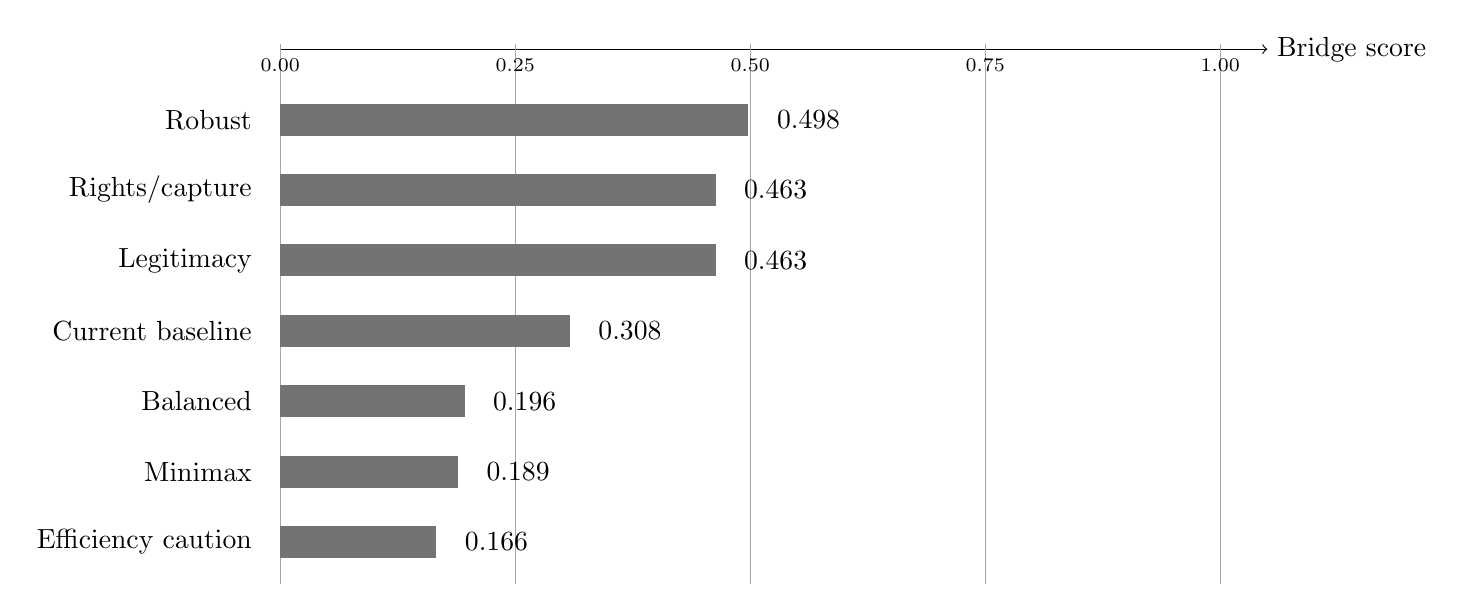
\begin{tikzpicture}[x=4.7in,y=0.80in]
\draw[->] (0,0) -- (1.05,0) node[anchor=west] {Bridge score};
\foreach \x/\lab in {0/0.00,0.25/0.25,0.50/0.50,0.75/0.75,1.00/1.00} {
  \draw[black!35] (\x,0.03) -- (\x,-3.34);
  \node[anchor=north] at (\x,0) {\scriptsize \lab};
}
\node[anchor=east] at (-0.02,-0.44) {Robust};
\fill[black!55] (0,-0.54) rectangle (0.498,-0.34);
\node[anchor=west] at (0.518,-0.44) {0.498};
\node[anchor=east] at (-0.02,-0.88) {Rights/capture};
\fill[black!55] (0,-0.98) rectangle (0.463,-0.78);
\node[anchor=west] at (0.483,-0.88) {0.463};
\node[anchor=east] at (-0.02,-1.32) {Legitimacy};
\fill[black!55] (0,-1.42) rectangle (0.463,-1.22);
\node[anchor=west] at (0.483,-1.32) {0.463};
\node[anchor=east] at (-0.02,-1.76) {Current baseline};
\fill[black!55] (0,-1.86) rectangle (0.308,-1.66);
\node[anchor=west] at (0.328,-1.76) {0.308};
\node[anchor=east] at (-0.02,-2.20) {Balanced};
\fill[black!55] (0,-2.30) rectangle (0.196,-2.10);
\node[anchor=west] at (0.216,-2.20) {0.196};
\node[anchor=east] at (-0.02,-2.64) {Minimax};
\fill[black!55] (0,-2.74) rectangle (0.189,-2.54);
\node[anchor=west] at (0.209,-2.64) {0.189};
\node[anchor=east] at (-0.02,-3.08) {Efficiency caution};
\fill[black!55] (0,-3.18) rectangle (0.166,-2.98);
\node[anchor=west] at (0.186,-3.08) {0.166};
\end{tikzpicture}
}
\caption{High-capture bridge scores across the focused bridge cases.}
\end{figure}


\section{Adaptive Survival Screen}

Adaptive Bridge v1 is a broader but more speculative screen. It runs \AdaptiveBridgeRunCount{} portfolio-stress simulations: every one of the \AdaptiveBridgePortfolioCount{} static portfolios under the \StressProfileCount{} stress profiles, for \AdaptiveBridgePeriodCount{} periods each. It keeps the v0 stress labels, then adds synthetic transition load, sequencing readiness, party adaptation, court adaptation, lobby venue shifting, emergency safeguards, federalism resistance, delivery bottlenecks, recovery capacity, voter feedback, and citizen agenda capacity.

This is not empirical validation. It is a skeptical institutional-survival screen. The Deep Research reports justify directional priors: narrow lobbying constraints invite venue shifting; emergency review matters only if it is fast, reason-giving, and anti-evasion oriented; high-complexity reforms need sequencing and administrative capacity; federalism and delivery bottlenecks are distinct failure modes; citizen agenda channels work best when deliberative and authenticated; and trust erosion is easier than trust recovery. The screen uses those priors to ask whether a portfolio still looks plausible after parties, courts, lobbyists, agencies, voters, and public agenda channels adapt.

The current adaptive leader is:

\begin{quote}
\AdaptiveLeaderName.
\end{quote}

Its average adaptive score is \AdaptiveLeaderScore, worst stress rank is \AdaptiveLeaderWorstStressRank, maximum adaptive stress regret is \AdaptiveLeaderMaxStressRegret, and the gate labels it \AdaptiveLeaderGate. The current run has \AdaptiveProvisionalShortlistCount{} provisional shortlist rows, \AdaptiveCalibrationGrayZoneCount{} calibration gray-zone rows, \AdaptiveReviewPriorityCount{} review-priority rows, and \AdaptiveDoNotRecommendCount{} rows marked do not recommend yet.

% Generated by paper/scripts/generate_tables.py; do not edit by hand.
\begin{table}[!htbp]
\centering
\small
\begin{tabular}{@{}L{0.26\linewidth}rL{0.55\linewidth}@{}}
\toprule
Adaptive gate & Count & Highest-ranked example \\
\midrule
provisional shortlist & 0 & none \\
calibration gray zone, not recommendation & 4,833 & Unicameral majority + pairwise alternatives + No emergency relief without merits review + Full anti-capture bundle (rank 1) \\
review priority, not recommendation & 0 & none \\
do not recommend yet & 29,019 & Citizen initiative and referendum + Pre-enactment constitutional council + Full anti-capture bundle (rank 135) \\
\bottomrule
\end{tabular}
\caption{Recommendation gate counts from Adaptive Bridge v1. Rows outside the provisional shortlist remain research targets rather than institutional recommendations.}
\end{table}


The important negative finding is that the static balanced winner does not survive this harsher adaptive screen. It falls to adaptive rank \BalancedAdaptiveRank, has average adaptive score \BalancedAdaptiveScore, worst stress rank \BalancedAdaptiveWorstStressRank, and maximum adaptive stress regret \BalancedAdaptiveMaxStressRegret. Its gate is \BalancedAdaptiveGate. That does not refute the static score; it means the static balanced winner depends on assumptions that become fragile when high capture, emergency abuse, low trust, noncompliance, and implementation overload are modeled as adaptive processes.

The robustness candidate is stronger under v1 but still not a recommendation. It ranks \RobustAdaptiveRank{} with average adaptive score \RobustAdaptiveScore{} and worst stress rank \RobustAdaptiveWorstStressRank; its gate is \RobustAdaptiveGate. The v1 result therefore shifts the paper's comparative focus from one balanced point-estimate winner to a family comparison: pairwise-alternatives and pairwise-tournament legislatures with emergency restraint and full anti-capture, audit, or voucher supports, plus portfolio-hybrid challengers retained by the static robustness diagnostics. That comparison is a research agenda, not a settled recommendation, because pairwise, portfolio-hybrid, and budgeted-lobbying families still need direct family-specific validation.

\section{Design Thesis}

Within this stylized evidence base, the most promising configured direction is not a minimalist majoritarian system or a maximal-review system. The emerging design direction is a moderated institutional portfolio:

\begin{itemize}
  \item a legislature with meaningful agenda access, alternative comparison, public-interest filtering, harm-sensitive safeguards, and active-law correction;
  \item a review system with enough independence to protect rights, strong emergency-restraint rules, and enough transparency to reduce legitimacy collapse;
  \item anti-capture rules that combine disclosure, public participation, enforcement, and evasion-aware monitoring without making ordinary advocacy impossible.
\end{itemize}

\section{Validation Agenda}

The current rows test institutional portfolios assembled from the imported simulators. Adaptive Bridge v1 now adds first-pass synthetic versions of transition load, implementation capacity, public feedback, citizen agenda channels, and adaptive political behavior. Those additions are useful, but they are still not deep enough to settle institutional recommendations. The next systems to model are speculative until they are implemented in source simulators, calibrated against evidence, and stress-tested as report artifacts.

% Generated by paper/scripts/generate_tables.py; do not edit by hand.
\begin{table}[!htbp]
\centering
\scriptsize
\begin{tabular}{@{}L{0.23\linewidth}L{0.54\linewidth}L{0.15\linewidth}@{}}
\toprule
Direction & Why add it & Claim status \\
\midrule
Phased reform sequences & Model transition paths rather than assuming all institutional changes arrive at once. & Speculative extension \\
Constitutional transition costs & Represent amendment difficulty, legitimacy shocks, retraining costs, litigation delay, and path-dependence. & Bridge v1 first-pass synthetic; needs calibration \\
Federalism and agency capacity & Add subnational veto points, administrative staffing, enforcement capacity, procurement pressure, and intergovernmental conflict. & Bridge v0/v1 stress layer; needs source simulator \\
Public implementation feedback & Let public trust, compliance, and perceived policy quality feed back into future agenda access and reform durability. & Bridge v1 first-pass synthetic; needs calibration \\
Citizen agenda setting & Test ballot access, deliberative citizen panels, public agenda petitions, and participatory budget channels as proposal-entry systems. & Bridge v1 first-pass synthetic; needs mechanism rows \\
\bottomrule
\end{tabular}
\caption{Systems and mechanisms that should be modeled next before stronger institutional recommendations are made.}
\end{table}


A credible future version should explain why a candidate survives adaptation by parties, courts, lobbyists, agencies, and voters. Parties may alter agenda strategy. Courts may change docket behavior. Lobbyists may shift venues and messengers. Agencies may fail to implement complex reforms. Voters may punish or reward outputs in ways that change compliance and legitimacy. Adaptive Bridge v1 now exposes its mechanism-family coefficients in configuration and reports, but those coefficients are still evidence-anchored priors rather than fitted causal estimates.

The highest-priority source refactor remains the review layer, but the first harmonization pass is now explicit. The updated Supreme Court Simulator Design paper warns against pooling pathway denominators, while the updated Constitutional Review Simulator exposes richer compliance and implementation outputs. The current harmonized source uses only shared static fields; future builds should either justify replacing source-specific metrics, move compliance and implementation variables into adaptive inputs, or keep the primary ranking source unchanged.

The current build reruns three review variants: the primary Supreme Court Design source, the companion Constitutional Review source, and the harmonized review source. The companion run produces \DualReviewCompanionPortfolioCount{} portfolios; only \DualReviewTopTwentyFiveOverlap{} of its top 25 portfolios overlap the current imported-review top 25, and the current primary winner's rank in the companion run is \DualReviewPrimaryWinnerRankInCompanion. The harmonized run produces \HarmonizedReviewPortfolioCount{} portfolios; only \HarmonizedReviewTopTwentyFiveOverlap{} of its top 25 portfolios overlap the current imported-review top 25, its top-100 overlap with the current run is \CurrentHarmonizedTopHundredOverlap, and the current primary winner ranks \HarmonizedReviewPrimaryWinnerRank{} in that run. The harmonized winner is \HarmonizedReviewWinnerName. This is evidence that review-source choice materially affects the shortlist.

% Generated by paper/scripts/generate_tables.py; do not edit by hand.
\begin{table}[!htbp]
\centering
\scriptsize
\resizebox{\linewidth}{!}{%
\begin{tabular}{@{}L{0.15\linewidth}L{0.16\linewidth}L{0.17\linewidth}r r r r r r L{0.28\linewidth}@{}}
\toprule
Run & Status & Review source & Scen. & Ports. & Score & Top-25 overlap & Primary winner rank & Run winner primary rank & Notes \\
\midrule
current-imported-review & completed & Supreme Court Simulator Design & 26 & 33852 & 0.656 & 25 & 1 & 1 & Current ranking source. \\
companion-review-first-pass & completed & Constitutional Review Simulator & 21 & 27342 & 0.673 & 2 & not comparable & not comparable & First-pass source swap; missing configured fields are skipped, not imputed. \\
harmonized-review-source & completed & Harmonized review source & 47 & 61194 & 0.671 & 2 & 265 & not comparable & Conservative harmonized source using only shared same-direction static review fields from both review projects. \\
\bottomrule
\end{tabular}
}
    \caption{Review-source static sensitivity. The companion run swaps in the Constitutional Review Simulator sensitivity campaign; the harmonized run uses only shared same-direction static review fields from both review projects. Overlap and rank columns use canonical portfolio keys with harmonized source prefixes stripped.}
    \end{table}

% Generated by paper/scripts/generate_tables.py; do not edit by hand.
\begin{table}[!htbp]
\centering
\small
\resizebox{\linewidth}{!}{%
\begin{tabular}{@{}L{0.18\linewidth}L{0.18\linewidth}r r r@{}}
\toprule
Left run & Right run & Top-25 overlap & Top-100 overlap & Shared canonical portfolios \\
\midrule
current & companion & 2 & 6 & 3,220 \\
current & harmonized & 2 & 6 & 43,470 \\
companion & harmonized & 19 & 86 & 33,810 \\
\bottomrule
\end{tabular}
}
\caption{Pairwise overlap among review-source variants. Counts use canonical portfolio keys, so harmonized rows from prefixed source scenarios can be compared to the corresponding source-run scenario when one exists.}
\end{table}

% Generated by paper/scripts/generate_tables.py; do not edit by hand.
\begin{table}[!htbp]
\centering
\scriptsize
\resizebox{\linewidth}{!}{%
\begin{tabular}{@{}r r r r r L{0.50\linewidth}@{}}
\toprule
Current & Companion & Harmonized & Comp.-cur. & Harm.-cur. & Portfolio \\
\midrule
-- & 2 & 1 & -- & -- & Expanded portfolio hybrid legislature + Mandatory legislative response cycles + Full anti-capture bundle \\
-- & 1 & 2 & -- & -- & Expanded portfolio hybrid legislature + Suspended declarations of invalidity + Full anti-capture bundle \\
1 & -- & 253 & -- & 252 & Expanded portfolio hybrid legislature + No emergency relief without merits review + Full anti-capture bundle \\
2 & -- & 257 & -- & 255 & Expanded portfolio hybrid legislature + Emergency integrity package + Full anti-capture bundle \\
-- & 3 & 8 & -- & -- & Expanded portfolio hybrid legislature + Weak-form review with legislative reply + Full anti-capture bundle \\
-- & 4 & 3 & -- & -- & Expanded portfolio hybrid legislature + Rights-impact statements before review + Full anti-capture bundle \\
3 & -- & 282 & -- & 279 & Expanded portfolio hybrid legislature + Automatic merits follow-up for emergency relief + Full anti-capture bundle \\
4 & -- & 310 & -- & 306 & Expanded portfolio hybrid legislature + Constitutional council with concrete-review backstop + Full anti-capture bundle \\
-- & 9 & 4 & -- & -- & Expanded portfolio hybrid legislature + Hybrid court balancing independence and accountability + Full anti-capture bundle \\
-- & 5 & 5 & -- & -- & Expanded portfolio hybrid legislature + Abstract review tribunal + Full anti-capture bundle \\
5 & 13 & 11 & 8 & 6 & Expanded portfolio hybrid legislature + Pre-enactment constitutional council + Full anti-capture bundle \\
-- & 6 & 9 & -- & -- & Expanded portfolio hybrid legislature + Pre-enactment review before laws take effect + Full anti-capture bundle \\
\bottomrule
\end{tabular}
}
\caption{Rank shifts for the best-observed portfolios across review-source variants. Blank cells mean the canonical review scenario is not available in that variant.}
\end{table}


The goal is not to eliminate politics. The goal is to make strategic behavior visible, channel it through contestable procedures, and prevent any one actor class from converting temporary advantage into durable institutional control.

A stronger future version needs external calibration before it can move from screening to recommendation. The minimum validation program is:

\begin{itemize}
  \item historical data on proposal access, amendment selection, enactment, correction, and repeal under different legislative rules;
  \item emergency docket timing, reason-giving, merits follow-up, rights-impact, and compliance data for review systems;
  \item lobbying venue-shifting, enforcement, disclosure, sanctions, public-finance, and dark-money adaptation data;
  \item federalism, agency-capacity, implementation-delay, and public-feedback data that can calibrate transition and overload parameters;
  \item validation cases where parties, courts, lobbyists, agencies, and voters visibly adapted to a reform;
  \item external coefficient ranges for the configured Adaptive Bridge v1 mechanism families rather than only directionally justified priors.
\end{itemize}

\section{Limitations}

This paper does not claim that the current scores are empirically validated estimates of real-world constitutional performance. The sibling simulators are stylized comparative tools. The cumulative harness is a synthesis layer over their outputs.

The updated sibling papers do not all enter the ranking in the same way. Congress and Lobby Capture updates change imported CSV inputs directly. Supreme Court Simulator Design remains the imported review source. The updated Constitutional Review Simulator is referenced but not ranked because treating two differently calibrated review projects as interchangeable would double-count review evidence and mask denominator differences.

Bridge v0 is also stylized. Its feedback equations are transparent and auditable through \path{config/interbranch-bridge-v0.json}, but they are not calibrated causal estimates. It uses portfolio diagnostics as inputs rather than rerunning the sibling simulators period by period.

Adaptive Bridge v1 is broader than v0 but not more empirically authoritative. Its equations and mechanism-family coefficients are transparent through \path{config/adaptive-bridge-v1.json} and its reports, but its party, court, lobby, agency, voter, transition, and citizen-agenda mechanisms remain evidence-anchored priors rather than fitted estimates. It should be used to demote fragile winners and identify research priorities, not to announce a settled constitutional design.

The new uncertainty and regret diagnostics are guardrails, not solutions. The uncertainty bands are synthetic and should not be quoted as statistical confidence intervals. Because \BalancedUncertaintyOverlapCount{} portfolio intervals overlap the balanced winner's interval, point-estimate rank should be treated as a screening device rather than a settled ranking. The minimax-regret table depends on the currently configured value profiles; a different profile set could change the regret ordering. The watchlist identifies fragility inside the current model, but it cannot discover mechanisms the model has not implemented.

The adjacent \texttt{../Civ Pro} project is not imported yet because it is currently a civil-procedure learning game rather than a government-performance campaign simulator. It should enter later only if it exports comparable access-to-justice, procedural fairness, litigation-cost, or rule-compliance metrics.

\section{Working Conclusion}

The strongest current conclusion is methodological and provisional. Methodologically, institutional portfolios should be ranked under multiple value profiles, checked for interval overlap, filtered by exact, epsilon, and uncertainty-aware Pareto rules, tested through feedback loops, rerun under explicit stress profiles, and then screened through adaptive-survival gates before design claims are made. Substantively, the current configured runs make single-rule fixes look weak. The balanced winner is the leading static point-estimate and lower-bound candidate, but it is not uncertainty-resolved and it fails the adaptive recommendation gate. The robustness and adaptive gray-zone leaders are better validation targets than final designs. No portfolio should be recommended as settled policy until the adaptive assumptions are calibrated against external evidence.

\appendix
\section{Technical Method Appendix}

\subsection{Static Portfolio Scoring}

The cumulative score is built from normalized subsystem diagnostics rather than from one raw simulator score. The importer first aggregates each source report by scenario key. It then computes component summaries from available columns only; missing source columns are skipped rather than imputed. The portfolio layer combines one legislature, one review design, and one anti-capture design into diagnostics for policy delivery, public alignment, rights safeguard, capture resistance, legitimacy, efficiency, complexity score, and resilience floor.

The balanced score is intentionally not pure throughput. Delivery and efficiency matter, but the score also rewards rights safeguards, capture resistance, legitimacy, public alignment, and subsystem floor. The floor term is conservative: a portfolio that performs well in two subsystems but collapses on rights, capture resistance, or complexity should not become the headline candidate merely because its average is high.

% Generated by paper/scripts/generate_tables.py; do not edit by hand.
\begin{table}[!htbp]
\centering
\scriptsize
\begin{tabular}{@{}L{0.22\linewidth}L{0.70\linewidth}@{}}
\toprule
Diagnostic & Formula summary \\
\midrule
Policy delivery & Mean of legislature productivity, welfare, public alignment, inverse gridlock, and inverse time-to-correct-bad-law when available. \\
Public alignment & Mean of legislative representative quality, legislative public alignment, legislative and review democratic responsiveness, anti-capture representation, and anti-capture public interest. \\
Rights safeguard & Mean of review rights protection, legal stability, stability-rights score, inverse shadow-docket abuse, inverse emergency legitimacy risk, inverse constitutional conflict, inverse weak public-mandate passage, and inverse concentrated-harm passage. \\
Capture resistance & Mean of anti-capture control, anti-capture success, detection, sanctions, transparency gain, inverse capture rate, inverse public-preference distortion, inverse hidden influence, inverse legislative lobby capture, and legislative anti-lobbying success. \\
Legitimacy & Mean of legislative legitimacy, review legitimacy, review public confidence, review legitimacy-control score, and anti-capture representation. \\
Complexity score & Mean of administrative feasibility, inverse administrative costs, inverse review institutional cost, inverse implementation complexity, anti-capture reform feasibility, and inverse anti-capture administrative cost. \\
Efficiency & 0.65 times policy delivery plus 0.35 times complexity score. \\
Resilience floor & Minimum of legislature component score, review component score, anti-capture component score, rights safeguard, capture resistance, and complexity score. \\
\bottomrule
\end{tabular}
\caption{Static portfolio diagnostic construction. Values are normalized to 0--1 before aggregation.}
\end{table}


\subsection{Profile Sensitivity}

The alternate profiles expose normative dependence in the rankings. The efficiency-first profile rewards delivery, implementation efficiency, and low complexity. The rights-first profile rewards rights safeguards, legal stability, legitimacy, and resilience floor. The anti-capture-first profile emphasizes capture resistance, public alignment, legitimacy, and transparency. The low-complexity profile emphasizes administrative tractability. The legitimacy-first profile emphasizes legitimacy, democratic/public alignment, rights safeguards, and capture resistance. A portfolio that wins only one profile is treated as a value-specific candidate; a portfolio that remains competitive across profiles is treated as a stronger design candidate.

% Generated by paper/scripts/generate_tables.py; do not edit by hand.
\begin{table}[!htbp]
\centering
\scriptsize
\begin{tabular}{@{}L{0.20\linewidth}L{0.72\linewidth}@{}}
\toprule
Profile & Weights \\
\midrule
Balanced & policyDelivery 22\%; publicAlignment 18\%; rightsSafeguard 18\%; captureResistance 18\%; legitimacy 10\%; efficiency 8\%; resilienceFloor 6\% \\
Efficiency First & policyDelivery 32\%; efficiency 26\%; complexityScore 18\%; publicAlignment 8\%; rightsSafeguard 6\%; captureResistance 6\%; legitimacy 4\% \\
Rights First & rightsSafeguard 36\%; legitimacy 18\%; publicAlignment 14\%; captureResistance 12\%; policyDelivery 8\%; resilienceFloor 8\%; efficiency 4\% \\
Anti-Capture First & captureResistance 38\%; publicAlignment 16\%; legitimacy 14\%; rightsSafeguard 10\%; policyDelivery 8\%; resilienceFloor 8\%; efficiency 6\% \\
Low Complexity & complexityScore 34\%; efficiency 20\%; resilienceFloor 14\%; policyDelivery 12\%; publicAlignment 8\%; rightsSafeguard 6\%; captureResistance 6\% \\
Legitimacy First & legitimacy 30\%; publicAlignment 24\%; rightsSafeguard 14\%; captureResistance 12\%; policyDelivery 8\%; complexityScore 6\%; resilienceFloor 6\% \\
\bottomrule
\end{tabular}
\caption{Scoring profile weights used for static reranking.}
\end{table}


% Generated by paper/scripts/generate_tables.py; do not edit by hand.
\begin{table}[!htbp]
\centering
\small
\begin{tabular}{@{}L{0.18\linewidth}L{0.55\linewidth}r r@{}}
\toprule
Profile & Winning portfolio & Score & Balanced rank \\
\midrule
Balanced & Expanded portfolio hybrid legislature + No emergency relief without merits review + Full anti-capture bundle & 0.656 & 1 \\
Efficiency First & Default pass unless 2/3 block + No emergency relief without merits review + Democracy vouchers & 0.727 & 348 \\
Rights First & Unicameral majority + pairwise alternatives + No emergency relief without merits review + Full anti-capture bundle & 0.665 & 125 \\
Anti-Capture First & Unicameral majority + pairwise alternatives + No emergency relief without merits review + Full anti-capture bundle & 0.635 & 125 \\
Low Complexity & Default pass unless 2/3 block + 60 percent invalidation threshold + Democracy vouchers & 0.723 & 645 \\
Legitimacy First & Unicameral majority + pairwise alternatives + No emergency relief without merits review + Full anti-capture bundle & 0.627 & 125 \\
\bottomrule
\end{tabular}
\caption{Profile-specific portfolio winners.}
\end{table}

% Generated by paper/scripts/generate_tables.py; do not edit by hand.
\begin{table}[!htbp]
\centering
\scriptsize
\begin{tabular}{@{}L{0.32\linewidth}rrrrrrr@{}}
\toprule
Focused case & B & Eff. & Rights & Cap. & Low-cx & Legit. & Regret \\
\midrule
balanced winner & 1 & 2,317 & 37 & 1 & 29,440 & 34 & 7,041 \\
Rights First winner & 155 & 4,813 & 1 & 3 & 5,704 & 1 & 1,741 \\
robustness winner & 256 & 4,910 & 10 & 7 & 4,192 & 5 & 1,848 \\
minimax-regret winner & 339 & 1,265 & 3,818 & 130 & 1,371 & 580 & 1 \\
Efficiency First winner & 433 & 1 & 10,423 & 730 & 5 & 1,486 & 52 \\
Low Complexity winner & 738 & 3 & 19,874 & 1,381 & 1 & 6,701 & 504 \\
current-system-ish baseline & 43,106 & 40,261 & 42,635 & 41,315 & 23,908 & 42,884 & 39,611 \\
\bottomrule
\end{tabular}
\caption{Profile-by-profile ranks for the focused candidate set. Lower ranks are better.}
\end{table}

% Generated by paper/scripts/generate_tables.py; do not edit by hand.
\begin{table}[!htbp]
\centering
\scriptsize
\begin{tabular}{@{}L{0.27\linewidth}r r r r r@{}}
\toprule
Case & Balanced rank & Score & Synthetic band & Half-width & Max regret \\
\midrule
balanced winner & 1 & 0.656 & 0.563--0.748 & 0.092 & 0.107 \\
Rights First winner & 125 & 0.640 & 0.548--0.733 & 0.092 & 0.083 \\
robustness winner & 267 & 0.635 & 0.542--0.727 & 0.092 & 0.086 \\
minimax-regret winner & 323 & 0.633 & 0.538--0.727 & 0.094 & 0.051 \\
Efficiency First winner & 348 & 0.631 & 0.533--0.730 & 0.098 & 0.061 \\
Low Complexity winner & 645 & 0.625 & 0.526--0.723 & 0.099 & 0.073 \\
current-system-ish baseline & 33,486 & 0.500 & 0.396--0.603 & 0.104 & 0.163 \\
\bottomrule
\end{tabular}
\caption{Uncertainty and regret diagnostics for the focused candidate set. Bands are synthetic model-sensitivity bands, not empirical confidence intervals.}
\end{table}

% Generated by paper/scripts/generate_tables.py; do not edit by hand.
\begin{table}[!htbp]
\centering
\scriptsize
\resizebox{\linewidth}{!}{%
\begin{tabular}{@{}r r r r L{0.58\linewidth}@{}}
\toprule
Regret rank & Max regret & Avg. regret & Balanced rank & Portfolio \\
\midrule
1 & 0.050 & 0.034 & 339 & Default pass + multi-round mediation + challenge + No emergency relief without merits review + Full anti-capture bundle \\
2 & 0.052 & 0.036 & 379 & Default pass + multi-round mediation + challenge + Automatic merits follow-up for emergency relief + Full anti-capture bundle \\
3 & 0.054 & 0.035 & 348 & Default pass + multi-round mediation + challenge + Emergency integrity package + Full anti-capture bundle \\
4 & 0.054 & 0.023 & 150 & Default pass unless 2/3 block + No emergency relief without merits review + Full anti-capture bundle \\
5 & 0.054 & 0.024 & 167 & Default pass unless 2/3 block + Emergency integrity package + Full anti-capture bundle \\
6 & 0.055 & 0.038 & 460 & Default pass + multi-round mediation + challenge + Randomized merits panels with en banc correction + Full anti-capture bundle \\
7 & 0.055 & 0.038 & 459 & Default pass + multi-round mediation + challenge + Three-judge panels with en banc correction + Full anti-capture bundle \\
8 & 0.055 & 0.039 & 472 & Default pass + multi-round mediation + challenge + Comparative 16-seat constitutional senates + Full anti-capture bundle \\
\bottomrule
\end{tabular}
}
\caption{Minimax-regret leaders across the configured value profiles. Low regret does not by itself make a portfolio recommendable.}
\end{table}


\subsection{Robustness and Pareto Filtering}

The robustness report is separate from the balanced report. Its score rewards low average profile rank, low worst profile rank, repeated top-profile appearances, limited score spread, and resilience floor. This is why the robustness winner can rank lower under the balanced score but remain central to the paper: it tests whether a design survives reasonable changes in value weighting.

The Pareto filter identifies portfolios that are not clearly dominated across the major diagnostics. It does not claim that every Pareto-front portfolio is equally plausible. Its role is narrower: it prevents the paper from discarding designs that are weaker on the headline score but stronger on a constitutionally important dimension such as rights, legitimacy, capture resistance, or complexity.

% Generated by paper/scripts/generate_tables.py; do not edit by hand.
\begin{table}[!htbp]
\centering
\small
\begin{tabular}{@{}L{0.30\linewidth}L{0.58\linewidth}@{}}
\toprule
Robustness diagnostic & Value \\
\midrule
Portfolio & Portfolio hybrid legislature + No emergency relief without merits review + Full anti-capture bundle \\
Robust score & 0.771 \\
Balanced rank & 256 \\
Average profile rank & 1563.333 \\
Worst profile rank & 4,910 \\
Top-25 profile appearances & 3 \\
\bottomrule
\end{tabular}
\caption{Cross-profile robustness winner.}
\end{table}

% Generated by paper/scripts/generate_tables.py; do not edit by hand.
\begin{table}[!htbp]
\centering
\scriptsize
\resizebox{\linewidth}{!}{%
\begin{tabular}{@{}r r r L{0.42\linewidth}L{0.38\linewidth}@{}}
\toprule
Balanced rank & Regret rank & Band & Portfolio & Do-not-recommend-yet reason \\
\midrule
1 & 7,041 & 0.092 & Expanded portfolio hybrid legislature + No emergency relief without merits review + Full anti-capture bundle & weak subsystem floor; weak public alignment; falls far under at least one value profile \\
2 & 7,578 & 0.092 & Expanded portfolio hybrid legislature + Emergency integrity package + Full anti-capture bundle & weak subsystem floor; weak public alignment; falls far under at least one value profile \\
3 & 7,278 & 0.092 & Expanded portfolio hybrid legislature + Automatic merits follow-up for emergency relief + Full anti-capture bundle & weak subsystem floor; weak public alignment; falls far under at least one value profile \\
4 & 8,163 & 0.093 & Expanded portfolio hybrid legislature + Constitutional council with concrete-review backstop + Full anti-capture bundle & weak subsystem floor; weak public alignment; falls far under at least one value profile \\
5 & 7,969 & 0.092 & Expanded portfolio hybrid legislature + Pre-enactment constitutional council + Full anti-capture bundle & weak subsystem floor; weak public alignment; falls far under at least one value profile \\
6 & 8,059 & 0.093 & Expanded portfolio hybrid legislature + Constitutional remand before invalidation + Full anti-capture bundle & weak subsystem floor; weak public alignment; falls far under at least one value profile \\
7 & 8,687 & 0.093 & Expanded portfolio hybrid legislature + Constitutional remand with override window + Full anti-capture bundle & weak subsystem floor; weak public alignment; falls far under at least one value profile \\
8 & 7,164 & 0.093 & Expanded portfolio hybrid legislature + Three-judge panels with en banc correction + Full anti-capture bundle & weak subsystem floor; weak public alignment; falls far under at least one value profile \\
\bottomrule
\end{tabular}
}
\caption{Fragile headline or near-headline portfolios that should not be converted into recommendations without more modeling.}
\end{table}

% Generated by paper/scripts/generate_tables.py; do not edit by hand.
\begin{table}[!htbp]
\centering
\small
\begin{tabular}{@{}L{0.42\linewidth}r@{}}
\toprule
Pareto diagnostic & Value \\
\midrule
Total generated portfolios & 43,470 \\
Exact point-estimate Pareto front & 2,730 (6.3\%) \\
Epsilon-Pareto front & 237 (0.5\%) \\
Uncertainty-aware Pareto front & 17,494 (40.2\%) \\
\bottomrule
\end{tabular}
\caption{Pareto-front sizes under exact, epsilon, and uncertainty-aware dominance rules.}
\end{table}


\subsection{Bridge Coefficients and Stress Profiles}

The bridge model is deterministic and configured through \path{config/interbranch-bridge-v0.json}. Its coefficients link legislative delivery, bad-policy inflow, review docket pressure, correction, court-curbing pressure, capture drift, public-alignment erosion, legitimacy, and compliance. The bridge does not rerun the sibling simulators period by period; it uses the portfolio diagnostics as initial conditions and feedback parameters.

The stress profiles are scenario multipliers over that same bridge. High-capture pressure raises starting capture and capture growth. Low-public-trust weakens starting legitimacy and compliance. High-rights-threat stress increases review pressure and quality plus backlog penalties. Court-curbing and noncompliance stress increases retaliation and compliance decay. Administrative-complexity stress reduces effective delivery, review capacity, and compliance. These stresses are not empirical forecasts; they are structured sensitivity checks over the same focused comparison set.

% Generated by paper/scripts/generate_tables.py; do not edit by hand.
\begin{table}[!htbp]
\centering
\scriptsize
\resizebox{\linewidth}{!}{%
\begin{tabular}{@{}rL{0.27\linewidth}rL{0.42\linewidth}@{}}
\toprule
Baseline bridge rank & Focused case & Static balanced rank & Selector \\
\midrule
1 & Balanced winner & 1 & cumulative-government-portfolios.csv rank 1 \\
2 & Efficiency caution case & 348 & profile-sensitivity.csv efficiency-first rank 1 \\
3 & Minimax-regret winner & 323 & portfolio-minimax-regret.csv rank 1 \\
4 & Rights/capture winner & 125 & profile-sensitivity.csv rights-first rank 1 \\
5 & Legitimacy-first winner & 125 & profile-sensitivity.csv legitimacy-first rank 1 \\
6 & Robustness winner & 267 & portfolio-robustness.csv rank 1 \\
7 & Current-system-ish baseline & 33,486 & fixed baseline keys \\
\bottomrule
\end{tabular}
}
\caption{Bridge v0 evaluates 7 focused cases from 33,852 static portfolios; 33,845 static portfolios are not bridge-simulated in the paper workflow.}
\end{table}

% Generated by paper/scripts/generate_tables.py; do not edit by hand.
\begin{table}[!htbp]
\centering
\footnotesize
\resizebox{\linewidth}{!}{%
\begin{tabular}{@{}rL{0.25\linewidth}r r r r r r@{}}
\toprule
Win/top-two rank & Case & Avg. rank & Worst & Wins & Top-two & Avg. score & Max regret \\
\midrule
1 & Balanced winner & 2.250 & 5 & 5 & 5 & 0.593 & 0.289 \\
2 & Robustness winner & 4.125 & 6 & 2 & 2 & 0.661 & 0.015 \\
3 & Rights/capture winner & 2.625 & 4 & 1 & 5 & 0.660 & 0.033 \\
4 & Efficiency caution case & 4.625 & 7 & 0 & 3 & 0.556 & 0.314 \\
5 & Legitimacy-first winner & 3.625 & 5 & 0 & 1 & 0.660 & 0.033 \\
6 & Minimax-regret winner & 4.125 & 6 & 0 & 0 & 0.570 & 0.298 \\
7 & Current-system-ish baseline & 6.625 & 7 & 0 & 0 & 0.379 & 0.483 \\
\bottomrule
\end{tabular}
}
\caption{Stress-profile stability across the focused bridge cases, sorted by the wins/top-two rule.}
\end{table}

% Generated by paper/scripts/generate_tables.py; do not edit by hand.
\begin{table}[!htbp]
\centering
\footnotesize
\begin{tabular}{@{}L{0.24\linewidth}L{0.28\linewidth}L{0.38\linewidth}@{}}
\toprule
Criterion & Winner & Winner metric \\
\midrule
Wins/top-two rule & Balanced winner & 5 wins; 5 top-two placements; average rank 2.250 \\
Best average stress rank & Balanced winner & average rank 2.250; worst rank 5 \\
Best average bridge score & Robustness winner & average bridge score 0.667 \\
Lowest maximum stress regret & Robustness winner & max stress regret 0.015; average regret 0.009 \\
Smallest score spread & Robustness winner & score spread 0.221 \\
\bottomrule
\end{tabular}
\caption{Alternative bridge-stability definitions. The wins/top-two rule is the default report sort, not the only stability interpretation.}
\end{table}

% Generated by paper/scripts/generate_tables.py; do not edit by hand.
\begin{table}[!htbp]
\centering
\small
\begin{tabular}{@{}L{0.42\linewidth}r@{}}
\toprule
Bridge-score component & Weight \\
\midrule
policyQuality & 22\% \\
legitimacy & 18\% \\
captureControl & 17\% \\
backlogControl & 14\% \\
compliance & 12\% \\
averageDelivery & 10\% \\
courtCurbingControl & 7\% \\
\bottomrule
\end{tabular}
\caption{Bridge-score weights from \texttt{config/interbranch-bridge-v0.json}.}
\end{table}

% Generated by paper/scripts/generate_tables.py; do not edit by hand.
\begin{table}[!htbp]
\centering
\scriptsize
\begin{tabular}{@{}L{0.26\linewidth}L{0.66\linewidth}@{}}
\toprule
Stress profile & Modifiers \\
\midrule
Baseline & none \\
High Capture Pressure & initialCapturePressureAdd=0.16; captureGrowthMultiplier=1.35; captureControlMultiplier=0.78; publicAlignmentCapturePenaltyMultiplier=1.25; legitimacyCapturePenaltyMultiplier=1.2; captureQualityPenaltyMultiplier=1.25 \\
Low Public Trust & baseLegitimacyMultiplier=0.82; initialComplianceAdd=-0.08; complianceMultiplier=0.9; legitimacyUncorrectedPenaltyMultiplier=1.25; legitimacyCapturePenaltyMultiplier=1.15; deliveryMultiplier=0.96 \\
High Rights-Threat Environment & badPolicyMultiplier=1.2; rightsThreatMultiplier=1.45; docketPressureMultiplier=1.2; badPolicyBacklogMultiplier=1.2; badPolicyQualityPenaltyMultiplier=1.25; netBenefitBadPolicyPenaltyMultiplier=1.2 \\
Court-Curbing and Institutional Noncompliance Stress & initialCourtCurbingPressureAdd=0.1; courtCurbingGrowthMultiplier=1.45; courtCurbingDecayMultiplier=0.65; complianceMultiplier=0.86; reviewCurbingPenaltyMultiplier=1.3; legitimacyCurbingPenaltyMultiplier=1.35; deliveryCourtCurbingPenaltyMultiplier=1.25 \\
Emergency Abuse Stress & initialCorrectionBacklogAdd=0.08; badPolicyMultiplier=1.16; rightsThreatMultiplier=1.38; docketPressureMultiplier=1.28; reviewCapacityMultiplier=0.92; badPolicyBacklogMultiplier=1.18; uncorrectedBacklogMultiplier=1.18; badPolicyQualityPenaltyMultiplier=1.2; legitimacyUncorrectedPenaltyMultiplier=1.32; netBenefitUncorrectedPenaltyMultiplier=1.2 \\
Administrative Overload and Complexity Stress & baseComplexityMultiplier=0.82; baseFloorMultiplier=0.92; deliveryMultiplier=0.92; reviewCapacityMultiplier=0.88; complianceMultiplier=0.92; captureGrowthMultiplier=1.08; docketPressureMultiplier=1.08 \\
Federalism and Agency-Capacity Stress & baseComplexityMultiplier=0.78; baseFloorMultiplier=0.9; deliveryMultiplier=0.88; reviewCapacityMultiplier=0.9; complianceMultiplier=0.84; captureGrowthMultiplier=1.12; docketPressureMultiplier=1.12; publicAlignmentUncorrectedPenaltyMultiplier=1.18; legitimacyUncorrectedPenaltyMultiplier=1.18; deliveryCourtCurbingPenaltyMultiplier=1.15 \\
\bottomrule
\end{tabular}
\caption{Bridge stress modifiers. Multipliers and additive adjustments are applied to the baseline bridge equations.}
\end{table}


\subsection{Adaptive Bridge v1}

Adaptive Bridge v1 is configured through \path{config/adaptive-bridge-v1.json}. It reuses the v0 stress profiles but expands the state vector to include transition load, sequencing readiness, strategic adaptation by parties, courts, and lobbyists, federalism resistance, delivery bottlenecks, recovery capacity, agency implementation gaps, voter feedback pressure, feedback correction capacity, emergency safeguards, and citizen agenda capacity. Its recommendation gate requires a strong average adaptive score, limited worst-stress rank, limited adaptive regret, bounded synthetic uncertainty, bounded profile regret, an adequate resilience floor, and enough direct evidence not to treat a thin family-specific result as recommendable.

The gate has four meanings. A provisional shortlist row passes the current synthetic screen but is still not an empirical recommendation. A calibration gray-zone row is strong enough to deserve direct validation but has unresolved evidence, stress, regret, or failure-mode caveats. A review-priority row is worth further modeling but fails more of the current gate conditions. A do-not-recommend-yet row should be treated as fragile under the present assumptions.

% Generated by paper/scripts/generate_tables.py; do not edit by hand.
\begin{table}[!htbp]
\centering
\small
\begin{tabular}{@{}L{0.88\linewidth}@{}}
\toprule
Synthetic adaptive mechanism introduced in Bridge v1 \\
\midrule
transition load from reform complexity, low subsystem floor, uncertainty, and profile regret \\
sequencing readiness from front-loaded legality, staffing, transparency, and review capacity \\
party adaptation and agenda obstruction \\
court adaptation and court-curbing pressure \\
lobby adaptation and venue shifting across agencies, courts, procurement, ballot campaigns, think tanks, and associations \\
agency implementation gaps under federalism resistance, delivery bottlenecks, and recovery capacity \\
public feedback through asymmetric trust erosion, voter backlash, compliance, and legitimacy \\
citizen agenda capacity as a corrective channel, with overload and rights-risk penalties for weakly deliberative tools \\
emergency-powers safeguards against fast, evasive, or normalized executive action \\
family-level direct-evidence strength used as a recommendation gate caveat \\
\bottomrule
\end{tabular}
\caption{Adaptive Bridge v1 mechanisms. These are transparent synthetic equations, not empirically calibrated parameters.}
\end{table}

% Generated by paper/scripts/generate_tables.py; do not edit by hand.
\begin{table}[!htbp]
\centering
\scriptsize
\begin{tabular}{@{}L{0.24\linewidth}L{0.68\linewidth}@{}}
\toprule
Calibration area & Use in Adaptive Bridge v1 \\
\midrule
Lobby venue shifting & Anti-capture rows with audit, machine-readable logs, venue-shift detection, or sanctions reduce lobby adaptation and capture pressure; narrow caps and budget tools keep a substitution-risk caveat. \\
Emergency powers & Emergency-integrity rows reduce rights-threat inflow, court adaptation, court-curbing pressure, and review backlog only when review is fast, reason-giving, and anti-evasion oriented. \\
Sequencing and transition costs & Sequencing readiness reduces transition load, agency gaps, and delivery bottlenecks; complex one-shot redesigns carry higher transition and direct-evidence penalties. \\
Federalism and agency capacity & The bridge now tracks federalism resistance, delivery bottleneck pressure, and recovery capacity separately before combining them into agency implementation gaps. \\
Public feedback & Feedback correction capacity can turn backlash into alignment and policy correction, while weak voice causes faster legitimacy erosion. \\
Citizen agenda setting & Citizen assemblies, random public review panels, and comment-authenticity rules improve agenda correction; initiatives and petition channels also add rights-risk or overload pressure. \\
Comparative evidence strength & Low-direct-evidence families can rank highly synthetically, but the recommendation gate labels them as calibration gray-zone or do-not-recommend rather than provisional recommendations. \\
\bottomrule
\end{tabular}
\caption{Evidence-informed priors added to Adaptive Bridge v1. The table records directional model use only; it is not an empirical fit.}
    \end{table}

% Generated by paper/scripts/generate_tables.py; do not edit by hand.
\begin{table}[!htbp]
\centering
\scriptsize
\resizebox{\linewidth}{!}{%
\begin{tabular}{@{}L{0.22\linewidth}L{0.16\linewidth}L{0.42\linewidth}L{0.24\linewidth}@{}}
\toprule
Coefficient family & Evidence tier & Additive coefficients & Multiplier coefficients \\
\midrule
audit-and-sanctions anti-capture & evidence-anchored prior & capCtrl=0.060; recovery=0.020; transReady=0.025 & lobbyAdapt=0.920 \\
venue-shifting detection & evidence-anchored prior & capCtrl=0.050; feedback=0.020; transReady=0.035 & lobbyAdapt=0.880 \\
democracy vouchers & evidence-informed prior & agendaCap=0.040; capCtrl=0.020; feedback=0.025 & lobbyAdapt=0.980 \\
budgeted disclosed lobbying & low-direct-evidence prior & capCtrl=0.025; capPress=0.012; transReady=0.010 & lobbyAdapt=0.980 \\
intermediary and dark-money substitution & evidence-anchored risk prior & agendaLoad=0.020; capPress=0.050 & lobbyAdapt=1.120 \\
emergency integrity & evidence-anchored prior & courtCurb=0.045; emergSafe=0.100; recovery=0.030; reviewCap=0.050; transReady=0.040 & -- \\
jurisdiction and pre-enactment review & evidence-informed prior & courtCurb=0.030; emergSafe=0.040; reviewCap=0.030; transReady=0.030 & -- \\
citizen assembly threshold & evidence-informed prior & agendaCap=0.070; agendaLoad=0.025; feedback=0.055; transReady=0.020 & partyAdapt=0.960 \\
random public review panel & evidence-informed prior & agendaCap=0.060; feedback=0.050; rightsRisk=-0.025 & partyAdapt=0.970 \\
citizens agenda petition & speculative-to-evidence-informed prior & agendaCap=0.060; agendaLoad=0.035; feedback=0.035 & partyAdapt=0.970 \\
citizen initiative referendum & risk-weighted prior & agendaCap=0.080; agendaLoad=0.050; capPress=0.020; feedback=0.025; rightsRisk=0.045 & -- \\
authenticated public participation & evidence-informed prior & agendaCap=0.035; capCtrl=0.030; feedback=0.035; transReady=0.020 & -- \\
pairwise alternatives & low-direct-evidence prior & deliverGap=0.015; feedback=0.025; transLoad=0.035 & partyAdapt=0.980 \\
portfolio hybrid & low-direct-evidence prior & deliverGap=0.020; transLoad=0.045; transReady=-0.020 & -- \\
default pass & risk-weighted prior & capPress=0.020; partyAdapt=0.020; rightsRisk=0.060 & -- \\
\bottomrule
\end{tabular}
}
\caption{Configured Adaptive Bridge v1 coefficient families. Coefficients are loaded from the v1 configuration and are evidence-anchored priors, not fitted causal estimates.}
\end{table}

% Generated by paper/scripts/generate_tables.py; do not edit by hand.
\begin{table}[!htbp]
\centering
\scriptsize
\resizebox{\linewidth}{!}{%
\begin{tabular}{@{}r r r r L{0.18\linewidth}L{0.20\linewidth}L{0.42\linewidth}@{}}
\toprule
Adaptive rank & Avg. score & Worst stress rank & Max regret & Evidence & Gate & Portfolio \\
\midrule
1 & 0.705 & 34 & 0.021 & mixed; low-direct-evidence family included & calibration gray zone, not recommendation & Unicameral majority + pairwise alternatives + No emergency relief without merits review + Full anti-capture bundle \\
2 & 0.704 & 37 & 0.022 & mixed; low-direct-evidence family included & calibration gray zone, not recommendation & Pairwise amendment tournament + majority + No emergency relief without merits review + Full anti-capture bundle \\
3 & 0.703 & 66 & 0.027 & mixed; low-direct-evidence family included & calibration gray zone, not recommendation & Unicameral majority + pairwise alternatives + Emergency integrity package + Full anti-capture bundle \\
4 & 0.703 & 70 & 0.028 & mixed; low-direct-evidence family included & calibration gray zone, not recommendation & Pairwise amendment tournament + majority + Emergency integrity package + Full anti-capture bundle \\
5 & 0.701 & 109 & 0.032 & low direct evidence & calibration gray zone, not recommendation & Unicameral majority + pairwise alternatives + Automatic merits follow-up for emergency relief + Full anti-capture bundle \\
6 & 0.700 & 116 & 0.033 & low direct evidence & calibration gray zone, not recommendation & Pairwise amendment tournament + majority + Automatic merits follow-up for emergency relief + Full anti-capture bundle \\
7 & 0.700 & 117 & 0.033 & mixed; low-direct-evidence family included & calibration gray zone, not recommendation & Portfolio hybrid legislature + No emergency relief without merits review + Full anti-capture bundle \\
8 & 0.698 & 346 & 0.020 & evidence-informed & calibration gray zone, not recommendation & Citizen initiative and referendum + No emergency relief without merits review + Full anti-capture bundle \\
9 & 0.698 & 184 & 0.039 & mixed; low-direct-evidence family included & calibration gray zone, not recommendation & Portfolio hybrid legislature + Emergency integrity package + Full anti-capture bundle \\
10 & 0.698 & 249 & 0.044 & low direct evidence & calibration gray zone, not recommendation & Unicameral majority + pairwise alternatives + Pre-enactment constitutional council + Full anti-capture bundle \\
\bottomrule
\end{tabular}
}
\caption{Adaptive Bridge v1 all-portfolio leaders. Gate status is a synthetic screening result, not a recommendation.}
\end{table}

% Generated by paper/scripts/generate_tables.py; do not edit by hand.
\begin{table}[!htbp]
\centering
\scriptsize
\resizebox{\linewidth}{!}{%
\begin{tabular}{@{}L{0.23\linewidth}L{0.55\linewidth}r r@{}}
\toprule
Stress profile & Adaptive winner & Score & Static rank \\
\midrule
Administrative Overload and Complexity Stress & Default pass unless 2/3 block + No emergency relief without merits review + Full anti-capture bundle & 0.687 & 119 \\
Baseline & Default pass unless 2/3 block + No emergency relief without merits review + Full anti-capture bundle & 0.742 & 119 \\
Court-Curbing and Institutional Noncompliance Stress & Default pass unless 2/3 block + No emergency relief without merits review + Full anti-capture bundle & 0.721 & 119 \\
Emergency Abuse Stress & Unicameral majority + pairwise alternatives + No emergency relief without merits review + Full anti-capture bundle & 0.739 & 125 \\
Federalism and Agency-Capacity Stress & Citizen initiative and referendum + No emergency relief without merits review + Full anti-capture bundle & 0.646 & 1,420 \\
High Capture Pressure & Unicameral majority + pairwise alternatives + No emergency relief without merits review + Full anti-capture bundle & 0.714 & 125 \\
High Rights-Threat Environment & Unicameral majority + pairwise alternatives + No emergency relief without merits review + Full anti-capture bundle & 0.740 & 125 \\
Low Public Trust & Default pass unless 2/3 block + No emergency relief without merits review + Full anti-capture bundle & 0.692 & 119 \\
\bottomrule
\end{tabular}
}
\caption{Stress-profile winners in Adaptive Bridge v1 over all static portfolios.}
\end{table}


\subsection{Input Provenance}

The paper build records hashes for the imported sibling simulator artifacts. The table below gives abbreviated hashes for print readability; the full SHA-256 values are written beside the generated LaTeX fragments.

% Generated by paper/scripts/generate_tables.py; do not edit by hand.
\begin{table}[!htbp]
\centering
\scriptsize
\begin{tabular}{@{}L{0.24\linewidth}r r L{0.31\linewidth}L{0.17\linewidth}@{}}
\toprule
Source & Rows & Scenarios & Imported report & SHA-256 prefix \\
\midrule
Congress Institutional Simulator & 1,702 & 46 & \texttt{simulation-\allowbreak{}campaign-\allowbreak{}v21-\allowbreak{}paper.csv} & \texttt{ec9cc17c99ccd290} \\
Supreme Court Simulator Design & 540 & 27 & \texttt{constitutional-\allowbreak{}review-\allowbreak{}campaign-\allowbreak{}v2.csv} & \texttt{7ba787af5a1143fa} \\
Lobby Capture Simulator & 35 & 35 & \texttt{lobby-\allowbreak{}capture-\allowbreak{}campaign.csv} & \texttt{1e517d7f62dc7395} \\
\bottomrule
\end{tabular}
\caption{Input source provenance for the current paper build. Full hashes are written to \texttt{paper/generated/source-provenance.json}.}
\end{table}


\end{document}
